
\documentclass[11pt,a4paper]{report}

\usepackage[portuges]{babel}
\usepackage[utf8]{inputenc} % define o encoding usado texto fonte (input)--usual "utf8" ou "latin1
\usepackage{graphicx} %permite incluir graficos, tabelas, figuras
\usepackage{subcaption}
\usepackage{listings}
\usepackage{color}
\usepackage{multicol}
\usepackage{indentfirst}
\usepackage{hyperref}
\usepackage{amsmath}
\usepackage{amssymb}

\definecolor{myblue}{rgb}{0.2,0.2,0.8}
\definecolor{mygray}{rgb}{0.5,0.5,0.5}
\definecolor{mymauve}{rgb}{0.58,0,0.82}

\lstdefinestyle{code}{ 
  backgroundcolor=\color{white},   % choose the background color; you must add \usepackage{color} or \usepackage{xcolor}; should come as last argument
  basicstyle=\footnotesize,        % the size of the fonts that are used for the code
  breakatwhitespace=false,         % sets if automatic breaks should only happen at whitespace
  breaklines=true,                 % sets automatic line breaking
  captionpos=b,                    % sets the caption-position to bottom
  commentstyle=\color{white},    % comment style
  deletekeywords={...},            % if you want to delete keywords from the given language
  escapeinside={\%*}{*)},          % if you want to add LaTeX within your code
  extendedchars=true,              % lets you use non-ASCII characters; for 8-bits encodings only, does not work with UTF-8
  firstnumber=1000,                % start line enumeration with line 1
  keepspaces=true,                 % keeps spaces in text, useful for keeping indentation of code (possibly needs columns=flexible)
  keywordstyle=\color{blue},       % keyword style
  language=C++,                 % the language of the code
  morekeywords={*,...},            % if you want to add more keywords to the set
  numberstyle=\tiny\color{mygray}, % the style that is used for the line-numbers
  rulecolor=\color{black},         % if not set, the frame-color may be changed on line-breaks within not-black text (e.g. comments (green here))
  showspaces=false,                % show spaces everywhere adding particular underscores; it overrides 'showstringspaces'
  showstringspaces=false,          % underline spaces within strings only
  showtabs=false,                  % show tabs within strings adding particular underscores
  stepnumber=2,                    % the step between two line-numbers. If it's 1, each line will be numbered
  stringstyle=\color{mymauve},     % string literal style
  tabsize=2,	                   % sets default tabsize to 2 spaces
  title=\lstname                   % show the filename of files included with \lstinputlisting; also try caption instead of title
}

\title{Interação e Concorrência (3º ano de Curso)\\
       \textbf{Teste}\\ Resolução
       } %Titulo do documento
%\title{Um Exemplo de Artigo em \LaTeX}
\author{ Ivo Lima\\ (A90214)
       } %autores do documento
\date{\today} %data

\begin{document}
	\begin{minipage}{0.9\linewidth}
        \centering
		
\includegraphics[width=0.4\textwidth]{um.jpeg}\par\vspace{1cm}
		{\scshape\LARGE Universidade do Minho} \par
		\vspace{0.6cm}
		{\scshape\Large Licenciatura em Ciências da Computação} \par
		\maketitle
	\end{minipage}


\tableofcontents % insere Indice

\chapter{Resolução das Questões}

\section{Questão 1}

\textbf{1.} 

\begin{figure} [h]
        \centering
		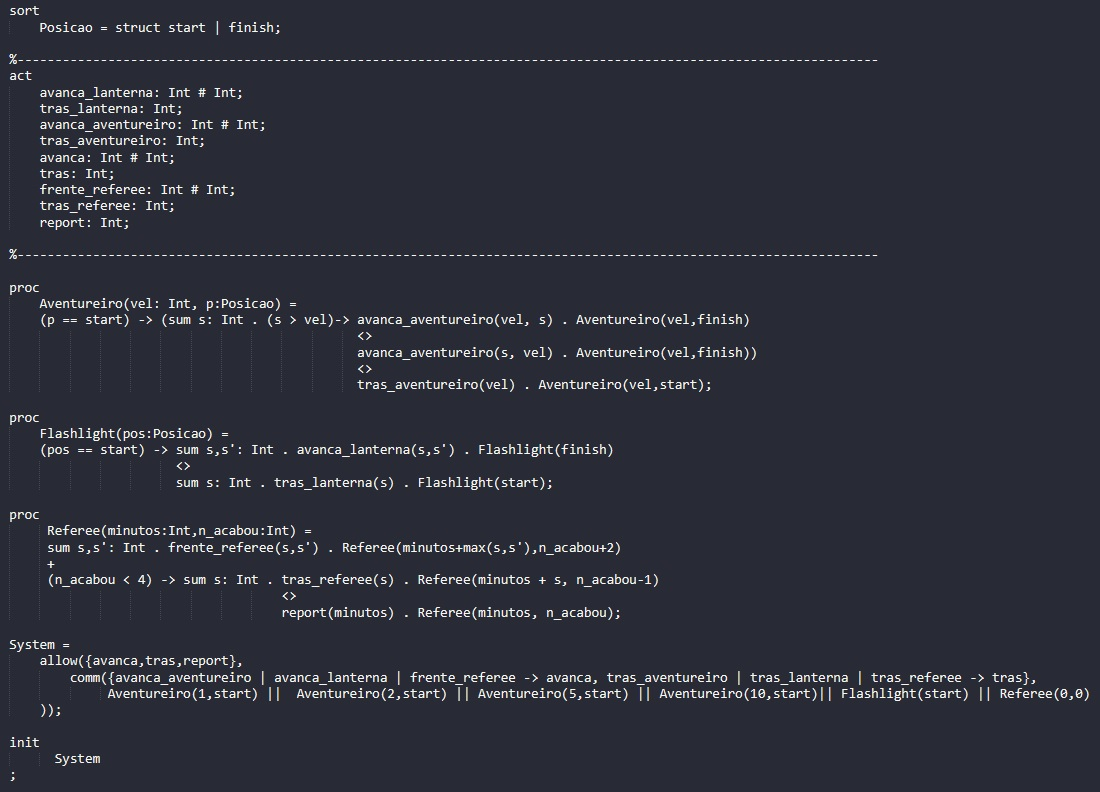
\includegraphics[width=0.90\textwidth]{Ex1.jpeg}\par\vspace{1cm}
\end{figure}

\begin{minipage}{0.9\linewidth}
        \centering
		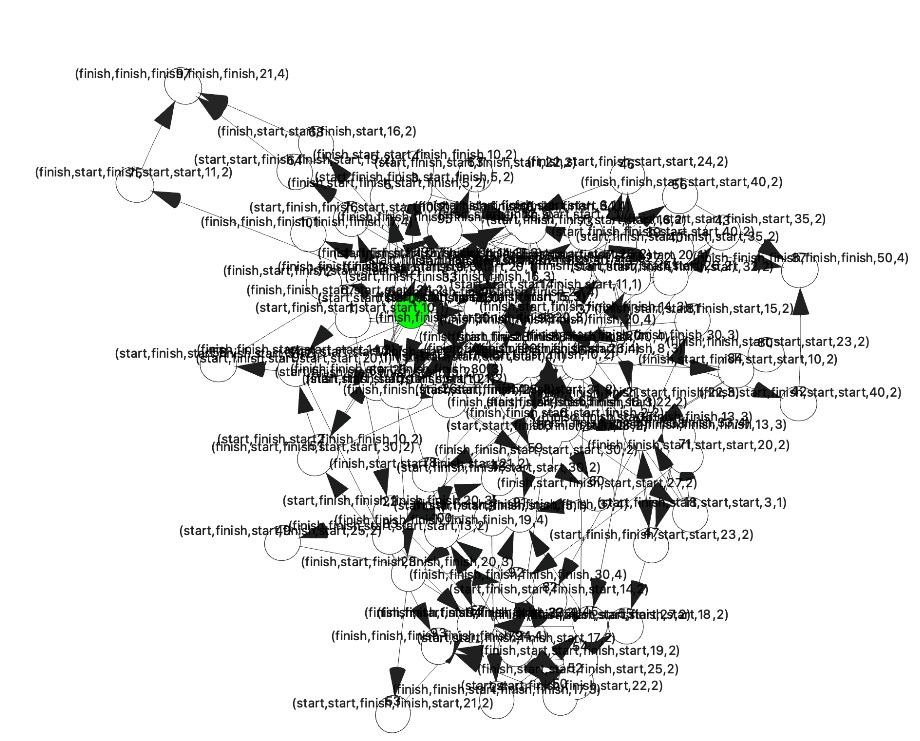
\includegraphics[width=\textwidth]{Ex11.jpeg}\par\vspace{1cm}
\end{minipage}

\newpage

\section{Questão 2}

Para realização desta questão foram utilizados o  documento apelidado como \emph{\href{https://www.researchgate.net/publication/30815544_The_Formal_Specification_Language_mCRL2}{The Formal Specification Language mCRL2}}, assim como o link \emph{\href{www.mcrl2.org/web/user_manual/tutorial/tutorial.html}{Tutoriais de mCRL2}} que foi disponibilizado pelo coordenador da disciplina.

Tendo em consideração aquilo que está escrito nos documentos acima indicados podemos assumir que o \emph{mCRL2} é uma linguagem de especificação formal, ou seja, deve ser usada durante uma fase de análise de requisitos e, de especificação de programas, descrevendo aquilo que deve ser feito e não como pois as especificações devem sofrer um processo de refinamento antes de serem implementadas de fato, isto é, a adição de detalhes de implementação. Assim como as outras linguagens de especificação é possibilitado a criação de provas matemáticas que validem ou revoguem o software. Para o efeito a mesma possui uma álgebra de processo genérica, baseada em Acp, o cálculo µ completo como uma lógica de especificação assim como um conjunto de ferramentas que lhe permitem  modelar, validar e verificar sistemas reativos e também protocolos concorrentes.

Depois deste breve apanhado sobre o que é e qual a funcionalidade da ferramenta \emph{mCRL2}, passaremos então a um exemplo da sua utilização. Para tal finalidade foi escolhido o seguinte caso \emph{\href{www.mcrl2.org/web/user_manual/tutorial/phonebook/index.html}{Lista telefônica}}.

Neste modelo foram impostos os seguintes requisitos:  \textbf{Armazenar um número de telefone}; \textbf{Adicionar e excluir entradas de uma lista telefônica}; \textbf{Apresentação de um número dado um nome}.

Atendendo as exigências colocadas podemos identificar as seguintes entidades: \textbf{Name}; \textbf{PhoneNumber}; \textbf{PhoneBook}. Em \emph{mCRL2} pode ser escrito da seguinte maneira:

\begin{lstlisting}
sort Name;
     PhoneNumber;
     PhoneBook = Name -> PhoneNumber;
\end{lstlisting}

Devemos ter em atenção que um nome pode não ter nenhum número de telefone associado, para lidarmos com esses casos criamos um número especial o \emph{p0}.

\begin{lstlisting}
map  p0: PhoneNumber; 
\end{lstlisting}

De seguida é necessário definir os parâmetros que as ações tomarão e como tal foram definidas as seguintes operações: \textbf{addPhone}; \textbf{delPhone}; \textbf{findPhone}. Deste modo:

\begin{lstlisting}
act  addPhone: Name # PhoneNumber;
     delPhone: Name;
     findPhone: Name;
\end{lstlisting}

\newpage
Tomando novamente em consideração a decisão anterior de criar um número especial \emph{p0}, para os nomes sem número associado, podemos ainda especificar que uma lista telefônica vazia mapeia todos os nomes para \emph{p0} numa fase inicial. Tal afirmação será representada do seguinte modo:

\begin{lstlisting}
lambda n: Name . p0;
\end{lstlisting}

Portanto na modelagem de uma lista telefônica vazia, podemos usar a abstração lambda. Na expressão estamos a definir uma função que recebe argumentos do tipo \emph{Name}, e produz para cada nome um \emph{p0} como resultado pois estes ainda não possuem nenhum número agregado a si. Uma vez que p0 é do tipo \emph{PhoneNumber},a expressão \emph{lambda n: Name . p0} descreve uma função do tipo \emph{Nome \textendash\textgreater PhoneNumber}, que por definição é igual a \emph{PhoneBook}. Dada uma função b do tipo \emph{PhoneBook}, um nome (n) e um número de telefone (p), podemos definir o valor de n em b para p usando a expressão \emph{b [n \textendash\textgreater p]}, desta maneira dizemos que todos os nomes \emph{m != n} , \emph{b [n \textendash\textgreater p] (m) = b (m)} e \emph{b [n \textendash\textgreater p] (n) = p}. 

Para além destes casos ainda temos de pensar em como impedir que seja atribuído a \emph{p0} todo e qualquer nome, o que pode ser facilmente evitado salvaguardando a ação \emph{addPhone} com \emph{p! = p0}. Logo após este pequeno problema temos um outro que é ter uma maneira efeciente de encontrar um dado número caso ele exista claro. Para tal existem duas abordagens possíveis:  \textbf{1.} Supor que o relatório do resultado é imediato e adicionar o número de telefone resultante como um parâmetro para a ação \emph{findPhone}, ou  \textbf{2.} Supor que a consulta de um número de telefone é assíncrona e, em seguida, dividir a consulta em ação iniciando a consulta (\emph{findPhone}) e uma ação relatando o resultado, por exemplo  \emph{reportPhone}.
Ambas as abordagens são adequadas pois na primeira situação é retratado um programa síncrono isto é, quando uma tarefa T1 inicia uma segunda tarefa T2, onde é garantido que o T2 seja iniciado e executado dentro do intervalo de tempo de T1 (existente) ou T1 "aguarda" o final de T2 e pode continuar o processamento posteriormente. Nesse sentido, T1 e T2 ocorrem "ao mesmo tempo" (não "em paralelo", mas em um intervalo de tempo contíguo), já na segunda circunstância é retratado um programa assíncrono isto é, o tempo de execução do T2 agora não está relacionado ao T1. Pode ser executado em paralelo, pode ocorrer um segundo, um minuto ou várias horas depois, e o T2 ainda pode ser executado quando o T1 terminar (para processar um resultado do T2, uma nova tarefa T3 pode ser necessária). Nesse sentido, T1 e T2 não estão a ocorrer ao mesmo tempo.

Utilização da 1º abordagem:

\begin{lstlisting}
proc PhoneDir(b: PhoneBook) = 
     sum n: Name, p: PhoneNumber . (p != p0) -> 
     addPhone(n, p) . PhoneDir(b[n->p])
     + sum n: Name . findPhone(n,b(n)) . PhoneDir()
     + sum n: Name . delPhone(n) . PhoneDir(b[n->p0]);
\end{lstlisting}

Para a utlização da 2º abordagem, deverá ser acrescentada uma nova ação e a 4º linha de \emph{PhoneDir} deverá ser substituída também.
\begin{lstlisting}
act  reportPhone: Name # PhoneNumber;

proc PhoneDir(b: PhoneBook) = 
     + sum n: Name.findPhone(n).reportPhone(n, b(n)).PhoneDir()
\end{lstlisting}

Ao verificarmos se o nosso ficheiro está está corretamente formado iremos obter a seguinte notificação \emph{'the file contains a well-formed mCRL2 specification'} e podemos então concluir que temos um especificação formal simples e correta para aquilo foi pedido inicialmente. Caso queiramos assegurar outras propriedades e ter em consideração um maior conjunto de ações, bem como outros problemas que possam aparecer a nossa específicação também irá crescer com ele. Possibilitando a realização de testes como o seguinte: apagar um número, encontrar um número, reportar um número, apagar novamente um número,verificar a lista telefónica, acrescentar um número, mudar um número,...

\begin{figure} [h]
        \centering
		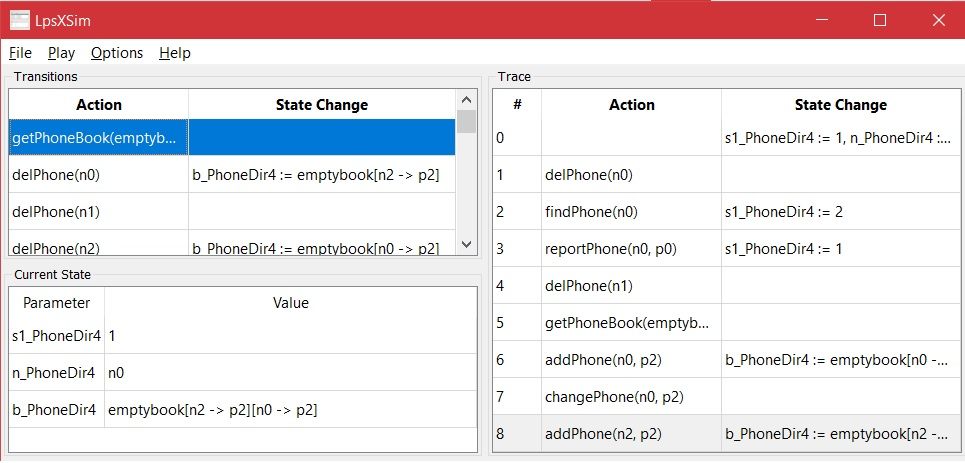
\includegraphics[width=0.60\textwidth]{Ex21.jpeg}\par\vspace{1cm}
\end{figure}
Podemos pedir à ferramenta um \emph{LTS} que é constituído por um conjunto de estados bem como um conjunto de transições entre esses estados, onde cada uma dessas transições é rotulada por uma ação e um estado é designado como o estado inicial.

\begin{figure} [h]
        \centering
		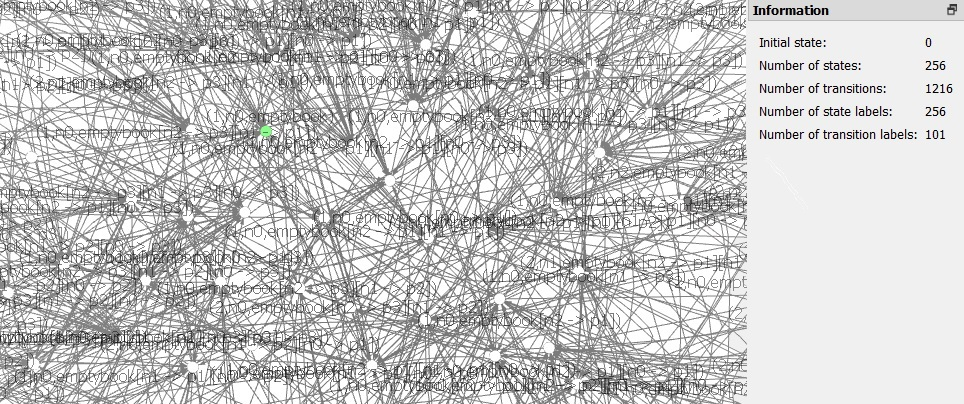
\includegraphics[width=0.70\textwidth]{Ex22.jpeg}\par\vspace{1cm}
\end{figure}

\section{Questão 3}

\textbf{3. a)} assim como a \textbf{3. b)}

\begin{minipage}{0.9\linewidth}
        \centering
		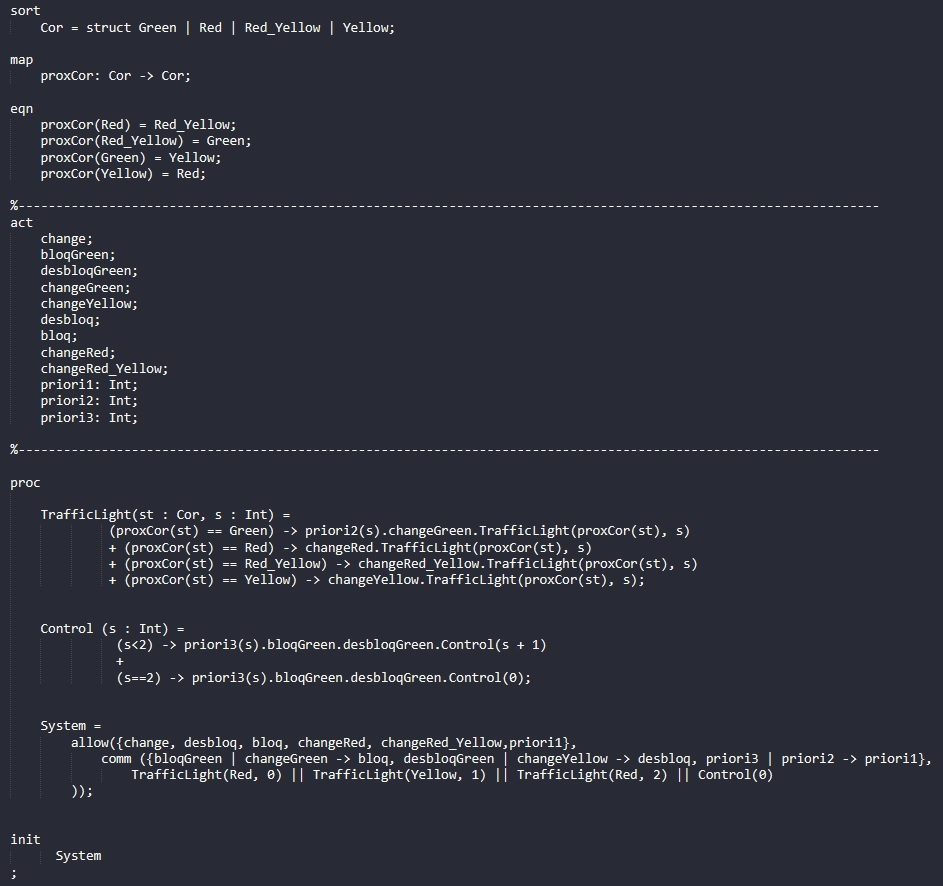
\includegraphics[width=\textwidth]{Ex3.jpeg}\par\vspace{1cm}
\end{minipage}

\textbf{3. c)}

Uma vez que \emph{X} é o meu \emph{Control}, este terá de considerar e controlar as diversas luzes segundo a prioridade \emph{A1 \textendash\textgreater  A2 \textendash\textgreater A3}, tendo isto em mente podemos atribuir a \emph{X} uma espécie de tuplo onde a alteração desses valores terá como efeito a alteração do estado que as luzes das estradas \emph{A1 A2} e \emph{A3} apresentam. 

\begin{minipage}{0.9\linewidth}
        \centering
		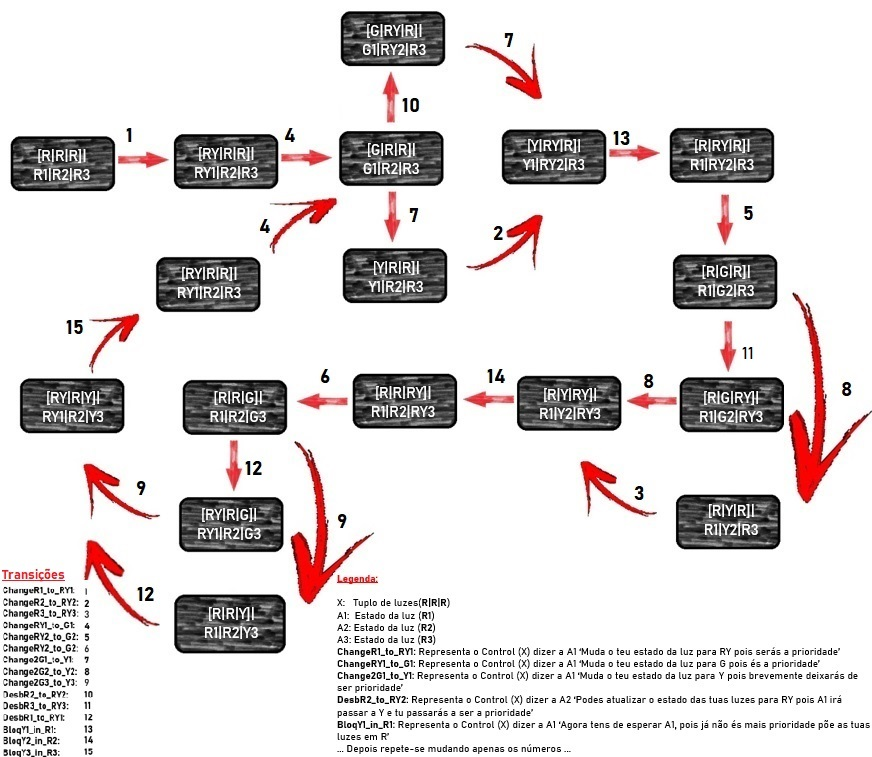
\includegraphics[width=\textwidth]{Ex33.jpeg}\par\vspace{1cm}
\end{minipage}

\textbf{3. d)}

\emph{A1=A2=A3 = R . RY . G . Y . R . RY . G...} sendo que neste é um ciclo repetitivo de ações irei omitir essa reescrita atribuindo um \emph{H} às mesmas. Logo \emph{A1=A2=A3 = R . RY . G . Y . H}.

\emph{X} terá o basto conjunto de ações enunciadas anteriormente e para não se tornar penosa a escrita de todas elas, estas serão representadas por um \emph{W}.

\begin{minipage}{0.75\linewidth}
        \centering
		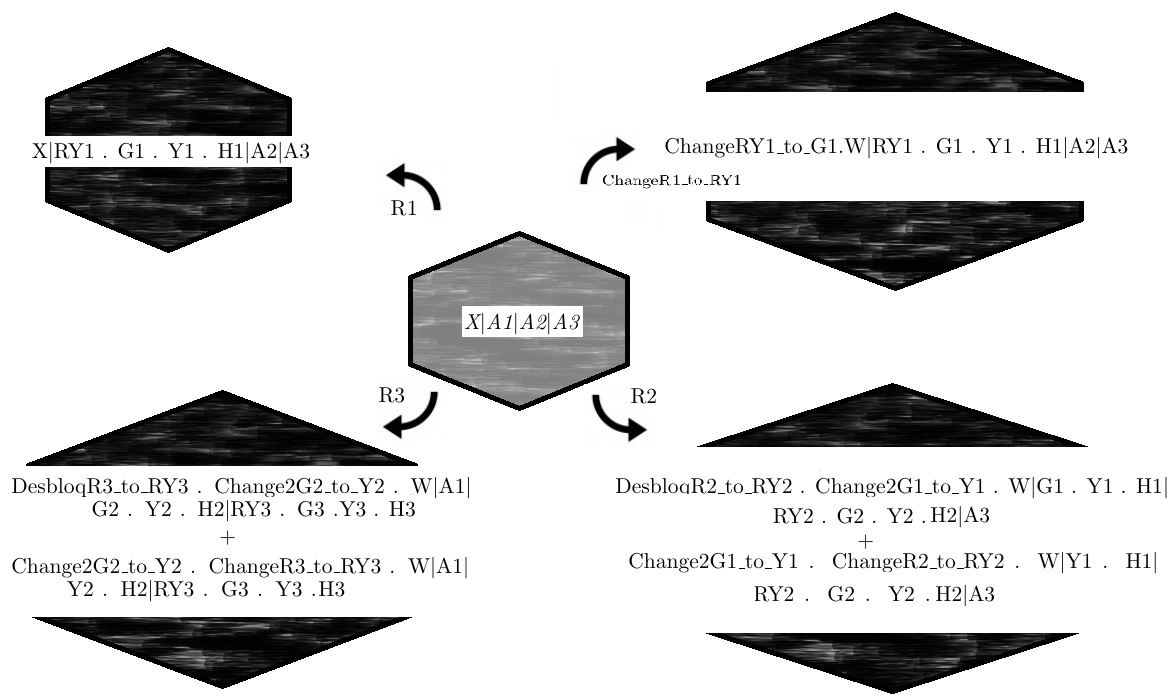
\includegraphics[width=\textwidth]{Ex34.jpeg}\par\vspace{1cm}
\end{minipage}

\textbf{(*)} \emph{X\textbar A1\textbar A2\textbar A3 $\sim$ X\textbar RY1 . G1 . Y1 . H1\textbar A2\textbar A3 + ChangeRY1\_to\_G1.W\textbar RY1 . G1 . Y1 . H1\textbar A2\textbar A3 + ... }

Portanto substitui processos exteriores paralelos por processos exteriores que são somas, sendo estas escolhas não determinísticas, onde os seus argumentos de derivação são \textbf{*} .

Analisando o resultado obtido aplicando o teorema podemos presumir que existe uma grande sincronização entre o processo \emph{X} e \emph{A1, A2, A3}, ou seja a dependência pedida na pergunta \textbf{3. b)} verificasse. Embora existam vários ramos possíveis continua a estar presente um certo ciclo o que pode significar a existência de uma única solução para o problema.

\section{Questão 4}

\textbf{4. a)}

\textbf{i.} 

A propriedade descrita nesta alínea é \textbf{falsa} e para tal basta apenas apresentar um contraexemplo que prove a falsidade da mesma. Se tomarmos como ponto de partida uma transição \emph{in} em  \emph{$U1\triangleright V1$} e tratando-se de uma \emph{bissimulação} o lado de \emph{$T\triangleright R$} também deverá conseguir fazer essa mesma transição, mas tal não acontece pois \emph{$T\triangleright R$} não têm na sua especificação nenhuma transição rotulada com \emph{in}, o mesmo aconteceria se pensássemos numa transição \emph{out}.

\textbf{ii.} 

Neste caso devemos ter em conta a definição de igualdade, que diz o seguinte 'a primeira transição $\tau$ deve ser correspondida em ambos os lados', isto é ser possível fazê-la tanto em \emph{$U2\triangleright V2$} como em \emph{$U1\triangleright V1$}. Para obtermos esse resultado temos de em ambos os casos recorrer à mudança das variáveis \emph{$\overline{out}$} e \emph{in} por \emph{$\bar{c}$} e \emph{c} respetivamente, feito isso podemos então realizar a transição por $\tau$. Logo podemos então neste momento comprovar que a definição foi respeitada e portanto somos capazes de \textbf{aprovar} a propriedade enunciada pelo exercício. 

\newpage

\textbf{4. b)}

\begin{minipage}{0.75\linewidth}
        \centering
		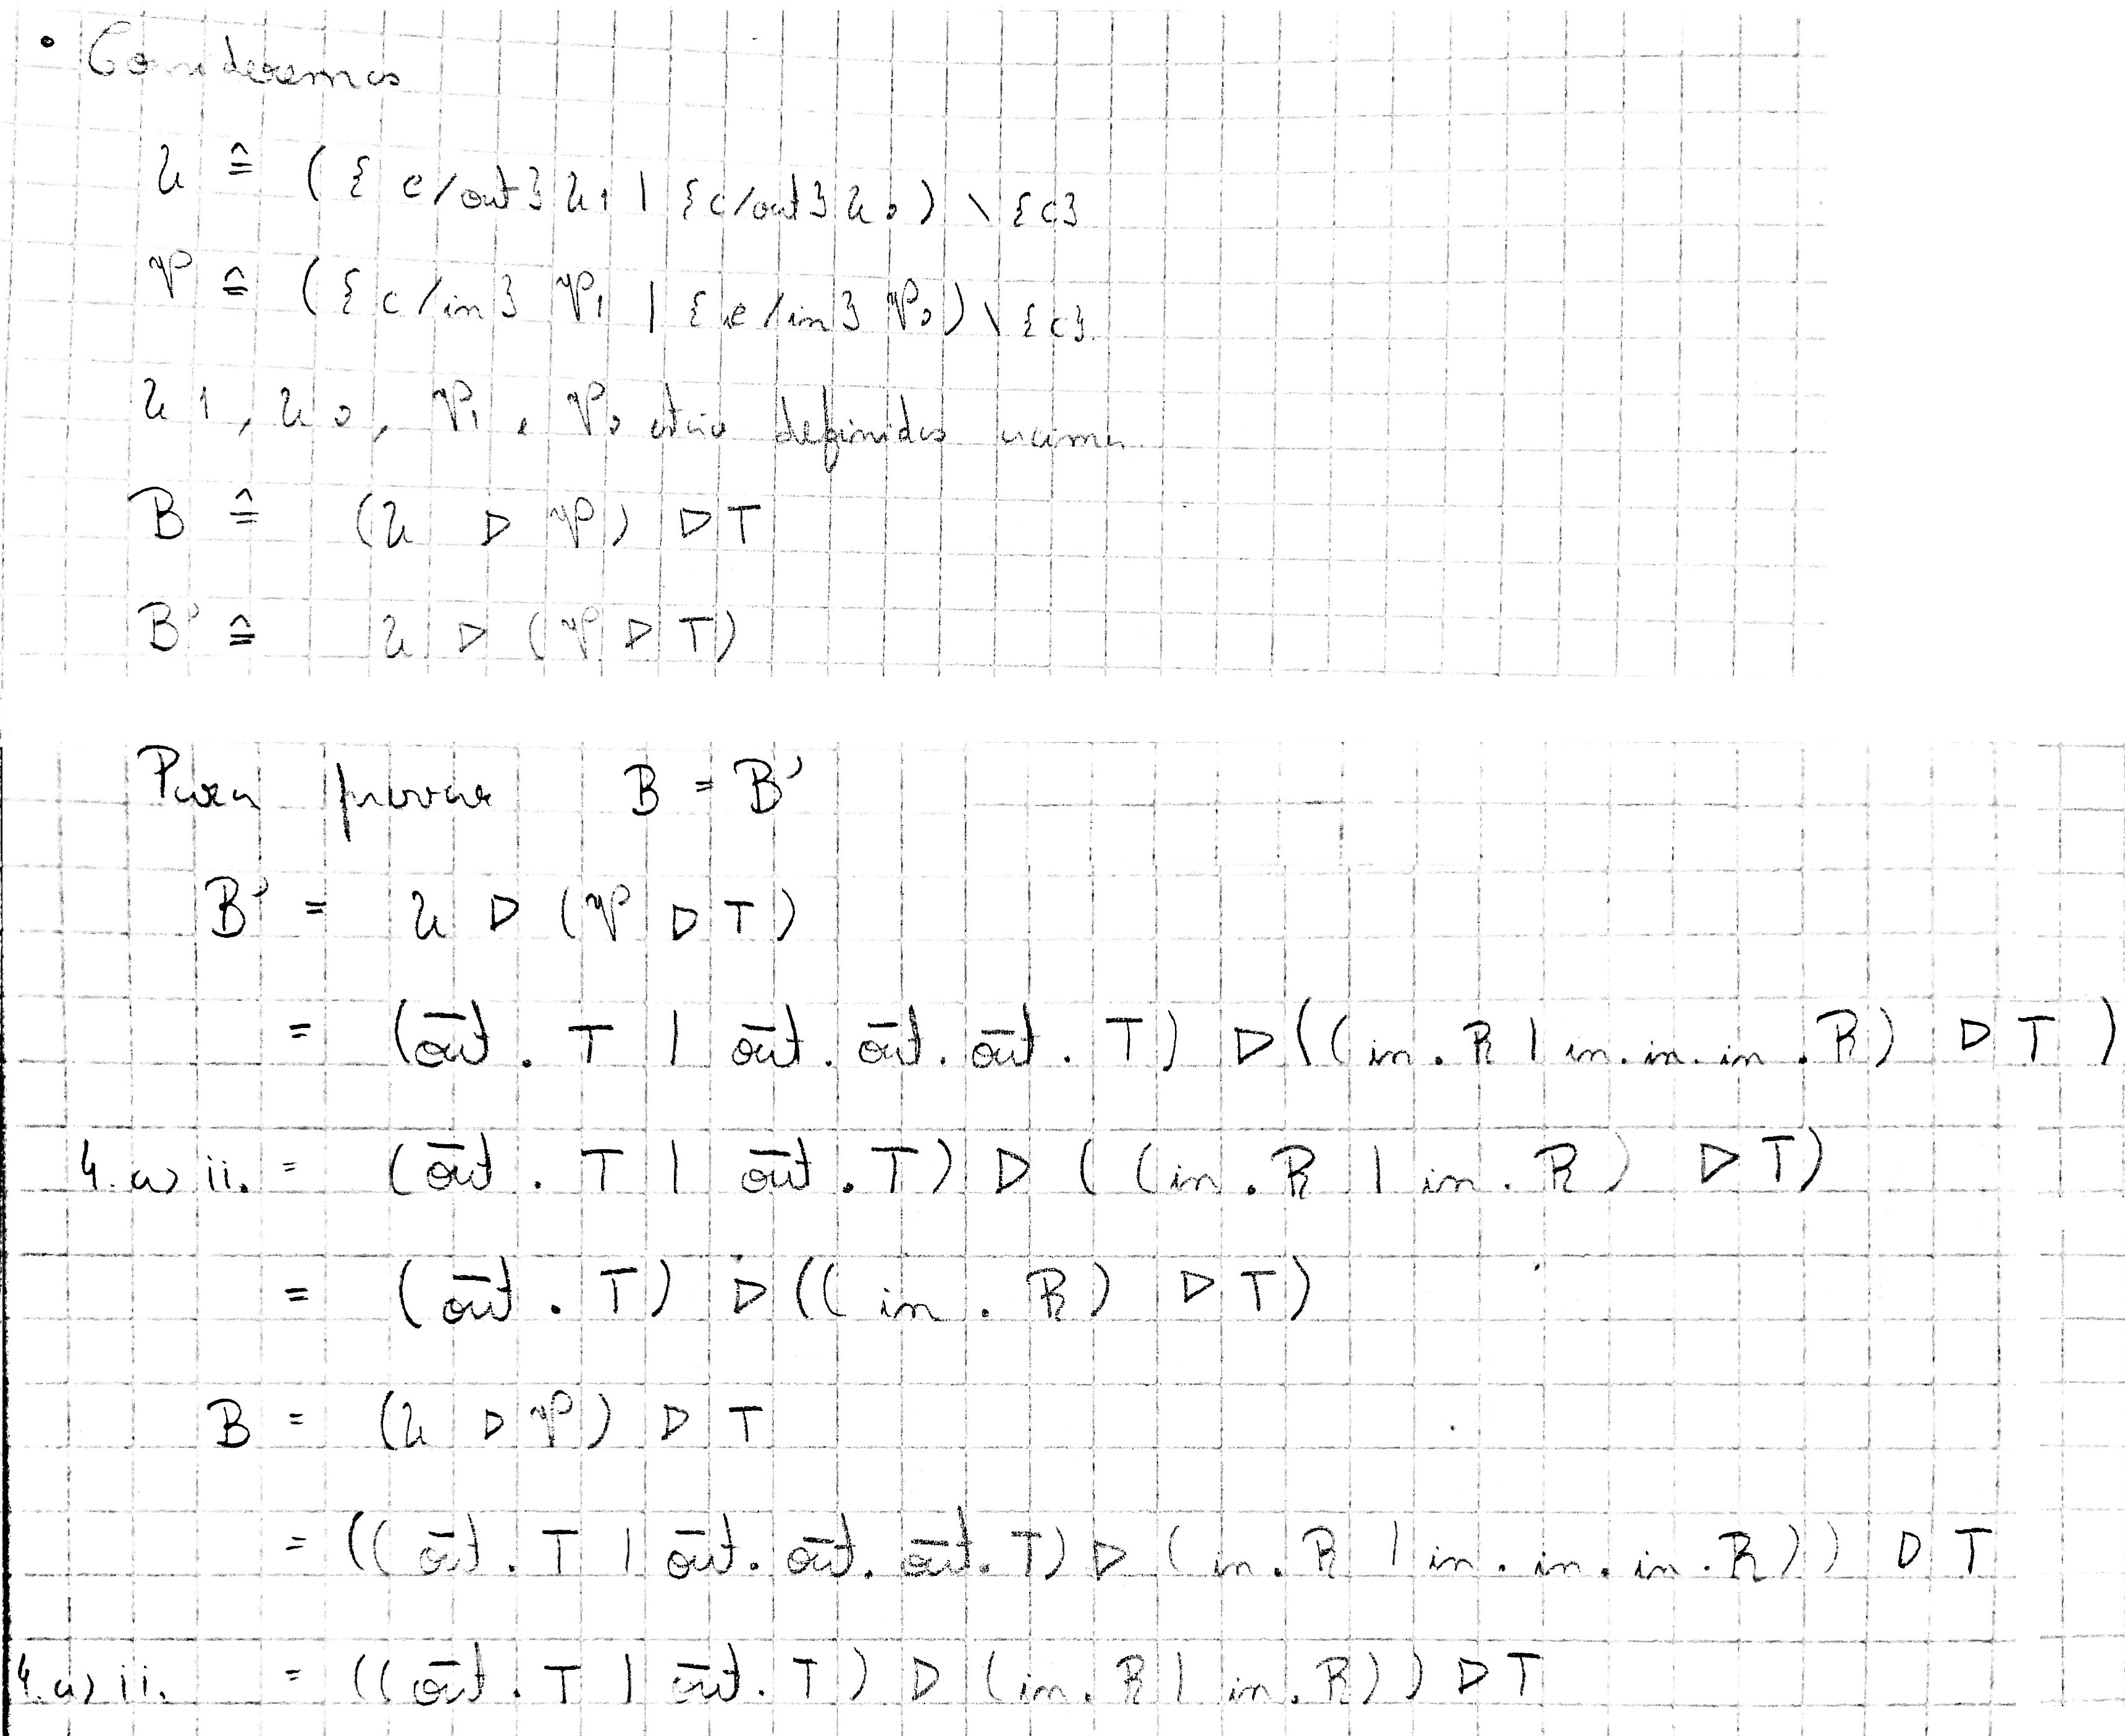
\includegraphics[width=\textwidth]{Ex4.jpeg}\par\vspace{1cm}
\end{minipage}

\textbf{4. c)}

Olhando para a definição que é apresentada no enunciado do exercício reparamos que \emph{U} e \emph{V} têm propriedades distintas, um pode fazer \emph{out's} ou substitui-los por \emph{c's} e o outro \emph{in's} ou substitui-los por \emph{c's}. Mas no contexto deste problema temos um único conjunto o \emph{0}, ou seja toda e qualquer propriedade que \emph{0} tenha será compartilhada consigo mesmo. Logo, ao querermos verificar-se \emph{$0\triangleright 0$} = \emph{0} este terá de respeitar a regra anteriormente enunciada de 'a primeira transição $\tau$ ser correspondida em ambos os lados' mas como estamos a falar do mesmo conjunto a imposição anterior será trivialmente respeitada e portanto a igualdade será verdade.
 
\section{Questão 5}

\textbf{5. a)} 

Através da análise das expressões reparamos que sempre que o processo $\circlearrowleft n \emph{E}$ tem capacidade de fazer uma transição por \emph{a} chegamos ao mesmo estado \emph{E} mas o seu n é decrementado e quando n toma o valor de 0, \emph{E} poderá fazer uma nova transição a que o levará a um novo estado \emph{E'}, ou seja neste ultima situação não é feito nada. Em suma podemos considerar o operador $\circlearrowleft$ uma espécie de \textbf{replicador}.

\newpage

\textbf{5. b)}

A expressão apresentada é \textbf{verdadeira} quando \emph{m} toma o valor de 0 e \emph{n} um valor natural qualquer como por exemplo 3, pois $\circlearrowleft 0 \emph{E}$ não irá alterar em nada \emph{E} (pois não acrescenta nem reduz o número de transições possíveis) e consequentemente $\circlearrowleft n \emph{E}$ será trivialmente bissimilar a $\circlearrowleft n \emph{E}$.

\textbf{5. c)}

Para fazermos a implicação pedida temos inicialmente de considerar o par R=\{($\circlearrowleft n \emph{E}$,$\circlearrowleft n \emph{F}$)\textbar E $\sim$ F\}, de seguida creiamos que existe em $\circlearrowleft n \emph{E}$ uma transição por \emph{a} para $\circlearrowleft n-1 \emph{E}$ então devido a E e F serem bissimilares tem de existir em $\circlearrowleft n \emph{F}$ uma transição por \emph{a} para $\circlearrowleft n-1 \emph{F}$, podemos abreviar todas estas transições por um simples $\sim$. Portanto ficaremos com um R=\{($\circlearrowleft n \emph{E}$,$\circlearrowleft n \emph{F}$)\textbar E $\sim$ F\} $\cup$ $\sim$. Porém a demonstração não pode ficar por aqui pois ainda temos os casos de existir em $\circlearrowleft 0 \emph{E}$ uma transição por \emph{a} para \emph{E'} bem como em $\circlearrowleft 0 \emph{F}$ haver uma transição por \emph{a} para \emph{F'} mas tal e qual como no exemplo acima apenas temos de adicionar estas transições a R. Em suma precisamos de ter R=\{($\circlearrowleft n \emph{E}$,$\circlearrowleft n \emph{F}$)\textbar E $\sim$ F\} $\cup$ $\sim$ $\cup$ \{(\emph{E'},\emph{F'})\textbar E $\sim$ F\} e assim conseguimos demonstrar que a implicação é \textbf{verdadeira}.

\textbf{5. d)} 

Se fizermos a troca de $\sim$ por $\approx$ tornaria a expressão anterior falsa, uma vez que nesse caso teriamos de analisar as transições \emph{"gordas"}, isto é $\circlearrowleft n \emph{E} \Rightarrow(a) \circlearrowleft n-1 \emph{E}$ assim 'a' pode ser uma transição simples que nesse caso acontecerá tanto em \emph{E} como \emph{F}, o problema surge quando 'a' for uma transição através de $\tau$ e dessa maneira acabamos quebrando a equivalência.

 $\circlearrowleft n \emph{E}$: $\tau$.x.0 $\rightarrow$($\tau$) $\tau$.$\tau$.x.0 $\rightarrow$($\tau$) ...

 $\circlearrowleft n \emph{F}$: x.x.0 $\rightarrow$(x) x.x.x.0 $\rightarrow(x)$ ...
 
\textbf{5. e)} 

Neste caso a solução é óbvia temos de forçar que o primeiro $\tau$ seja correspondido por outro $\tau$ ou levar a que quando um $\tau$ é feito \emph{E} ficar igual a \emph{F}, ou o contrário \emph{F} ficar igual a \emph{E}.
Tendo em conta que \emph{E $\neq$ $\tau$.E}, mas que \emph{$\tau$.E = $\tau$.$\tau$.E} podemos alterar a semântica do problema para:

\begin{figure} [h]
        \centering
		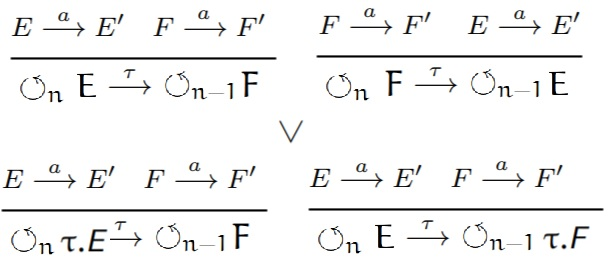
\includegraphics[width=0.70\textwidth]{Ex5.jpeg}\par\vspace{1cm}
\end{figure}

\end{document}